% ============================================================
% Conteúdo acadêmico puro do documento "Casos de Uso do Sistema".
% SEM \documentclass, \begin{document}/\end{document} nem título —
% pensado para ser reaproveitado via \input{} tanto no documento
% modular quanto, futuramente, no TCC principal.
%
% Fonte do conteúdo: Casos_de_Uso.md e Diagrama_Casos_de_Uso.puml
% (nesta mesma pasta), levantados a partir dos requisitos funcionais
% revisados, da Matriz_de_Rastreabilidade.md e de leitura direta do
% código-fonte (Services/PermissionService.cs) para confirmar atores
% e regras de permissão.
% ============================================================

\section{Apresentação}

Este documento especifica os casos de uso do sistema \textbf{RadarTorres}, complementando o
diagrama \texttt{Diagrama\_Casos\_de\_Uso.puml} com o detalhamento de cada caso de uso: atores
envolvidos e requisito(s) funcional(is) associado(s). Serve de ponte entre os requisitos
funcionais/não funcionais consolidados em \emph{Requisitos Funcionais e Não Funcionais} e o
comportamento observável do sistema (como um ator interage com ele para atingir um objetivo).

Nenhum caso de uso foi incluído sem lastro em um requisito funcional válido. Casos de uso
puramente automáticos (reação do sistema, sem ator humano nem Arduino diretamente ligados) —
Rastrear alvos, Selecionar torre automaticamente, Acompanhar alvo pelas torres, Executar
acionamento demonstrativo automático, Validar regras de segurança — não têm ator próprio: são
alcançados só via \emph{include}/\emph{extend} a partir de "Monitorar radar" (Usuário) e
"Receber/detectar alvos" (Arduino), reforçando que não há acionamento manual no sistema.

\section{Atores}

\begin{longtable}{p{2.4cm}p{11.6cm}}
  \caption{Atores do sistema RadarTorres} \\
  \hline
  \textbf{Ator} & \textbf{Descrição / Responsabilidades} \\
  \hline
  \endfirsthead
  \multicolumn{2}{c}{\small \tablename~\thetable\ (continuação)} \\
  \hline
  \textbf{Ator} & \textbf{Descrição / Responsabilidades} \\
  \hline
  \endhead
  \hline
  \endfoot
  \small
  Usuário (genérico) & Ator abstrato que representa qualquer perfil autenticado (Administrador,
  Operador e Visualizador herdam dele). Cobre autenticação, troca da própria senha, visualização
  do painel e do radar, consulta/exportação de histórico, preferências pessoais, abertura de
  chamado de ajuda e uso da aba de configuração do Arduino. \\
  Administrador & Acesso administrativo completo: gerenciar usuários, gerenciar zonas mortas,
  gerenciar chamados de ajuda, além de alterar modo de operação e importar objetos detectados. \\
  Operador & Perfil operacional sem acesso às telas administrativas: além do que \emph{Usuário}
  cobre, pode alterar modo de operação e importar objetos detectados. \\
  Visualizador & Perfil somente-consulta, restrito ao conjunto herdado de \emph{Usuário}; não
  pode alterar modo de operação, importar dados nem gerenciar usuários/zonas mortas/chamados. \\
  Arduino & Ator externo (hardware): envia leituras de ângulo/distância pela porta serial e é a
  origem das mensagens do monitor serial da aba de configuração. \\
\end{longtable}

\section{Diagrama de Casos de Uso}

O diagrama representa o sistema como uma única fronteira "Sistema RadarTorres", subdividida em 6
agrupamentos visuais para manter a legibilidade: \textbf{Conta e Acesso}, \textbf{Monitoramento e
Operação}, \textbf{Histórico e Dados}, \textbf{Administração}, \textbf{Preferências} e
\textbf{Arduino e Comunicação}. Fonte: \texttt{Diagrama\_Casos\_de\_Uso.puml} (PlantUML), nesta
mesma pasta.

\begin{figure}[htbp]
  \centering
  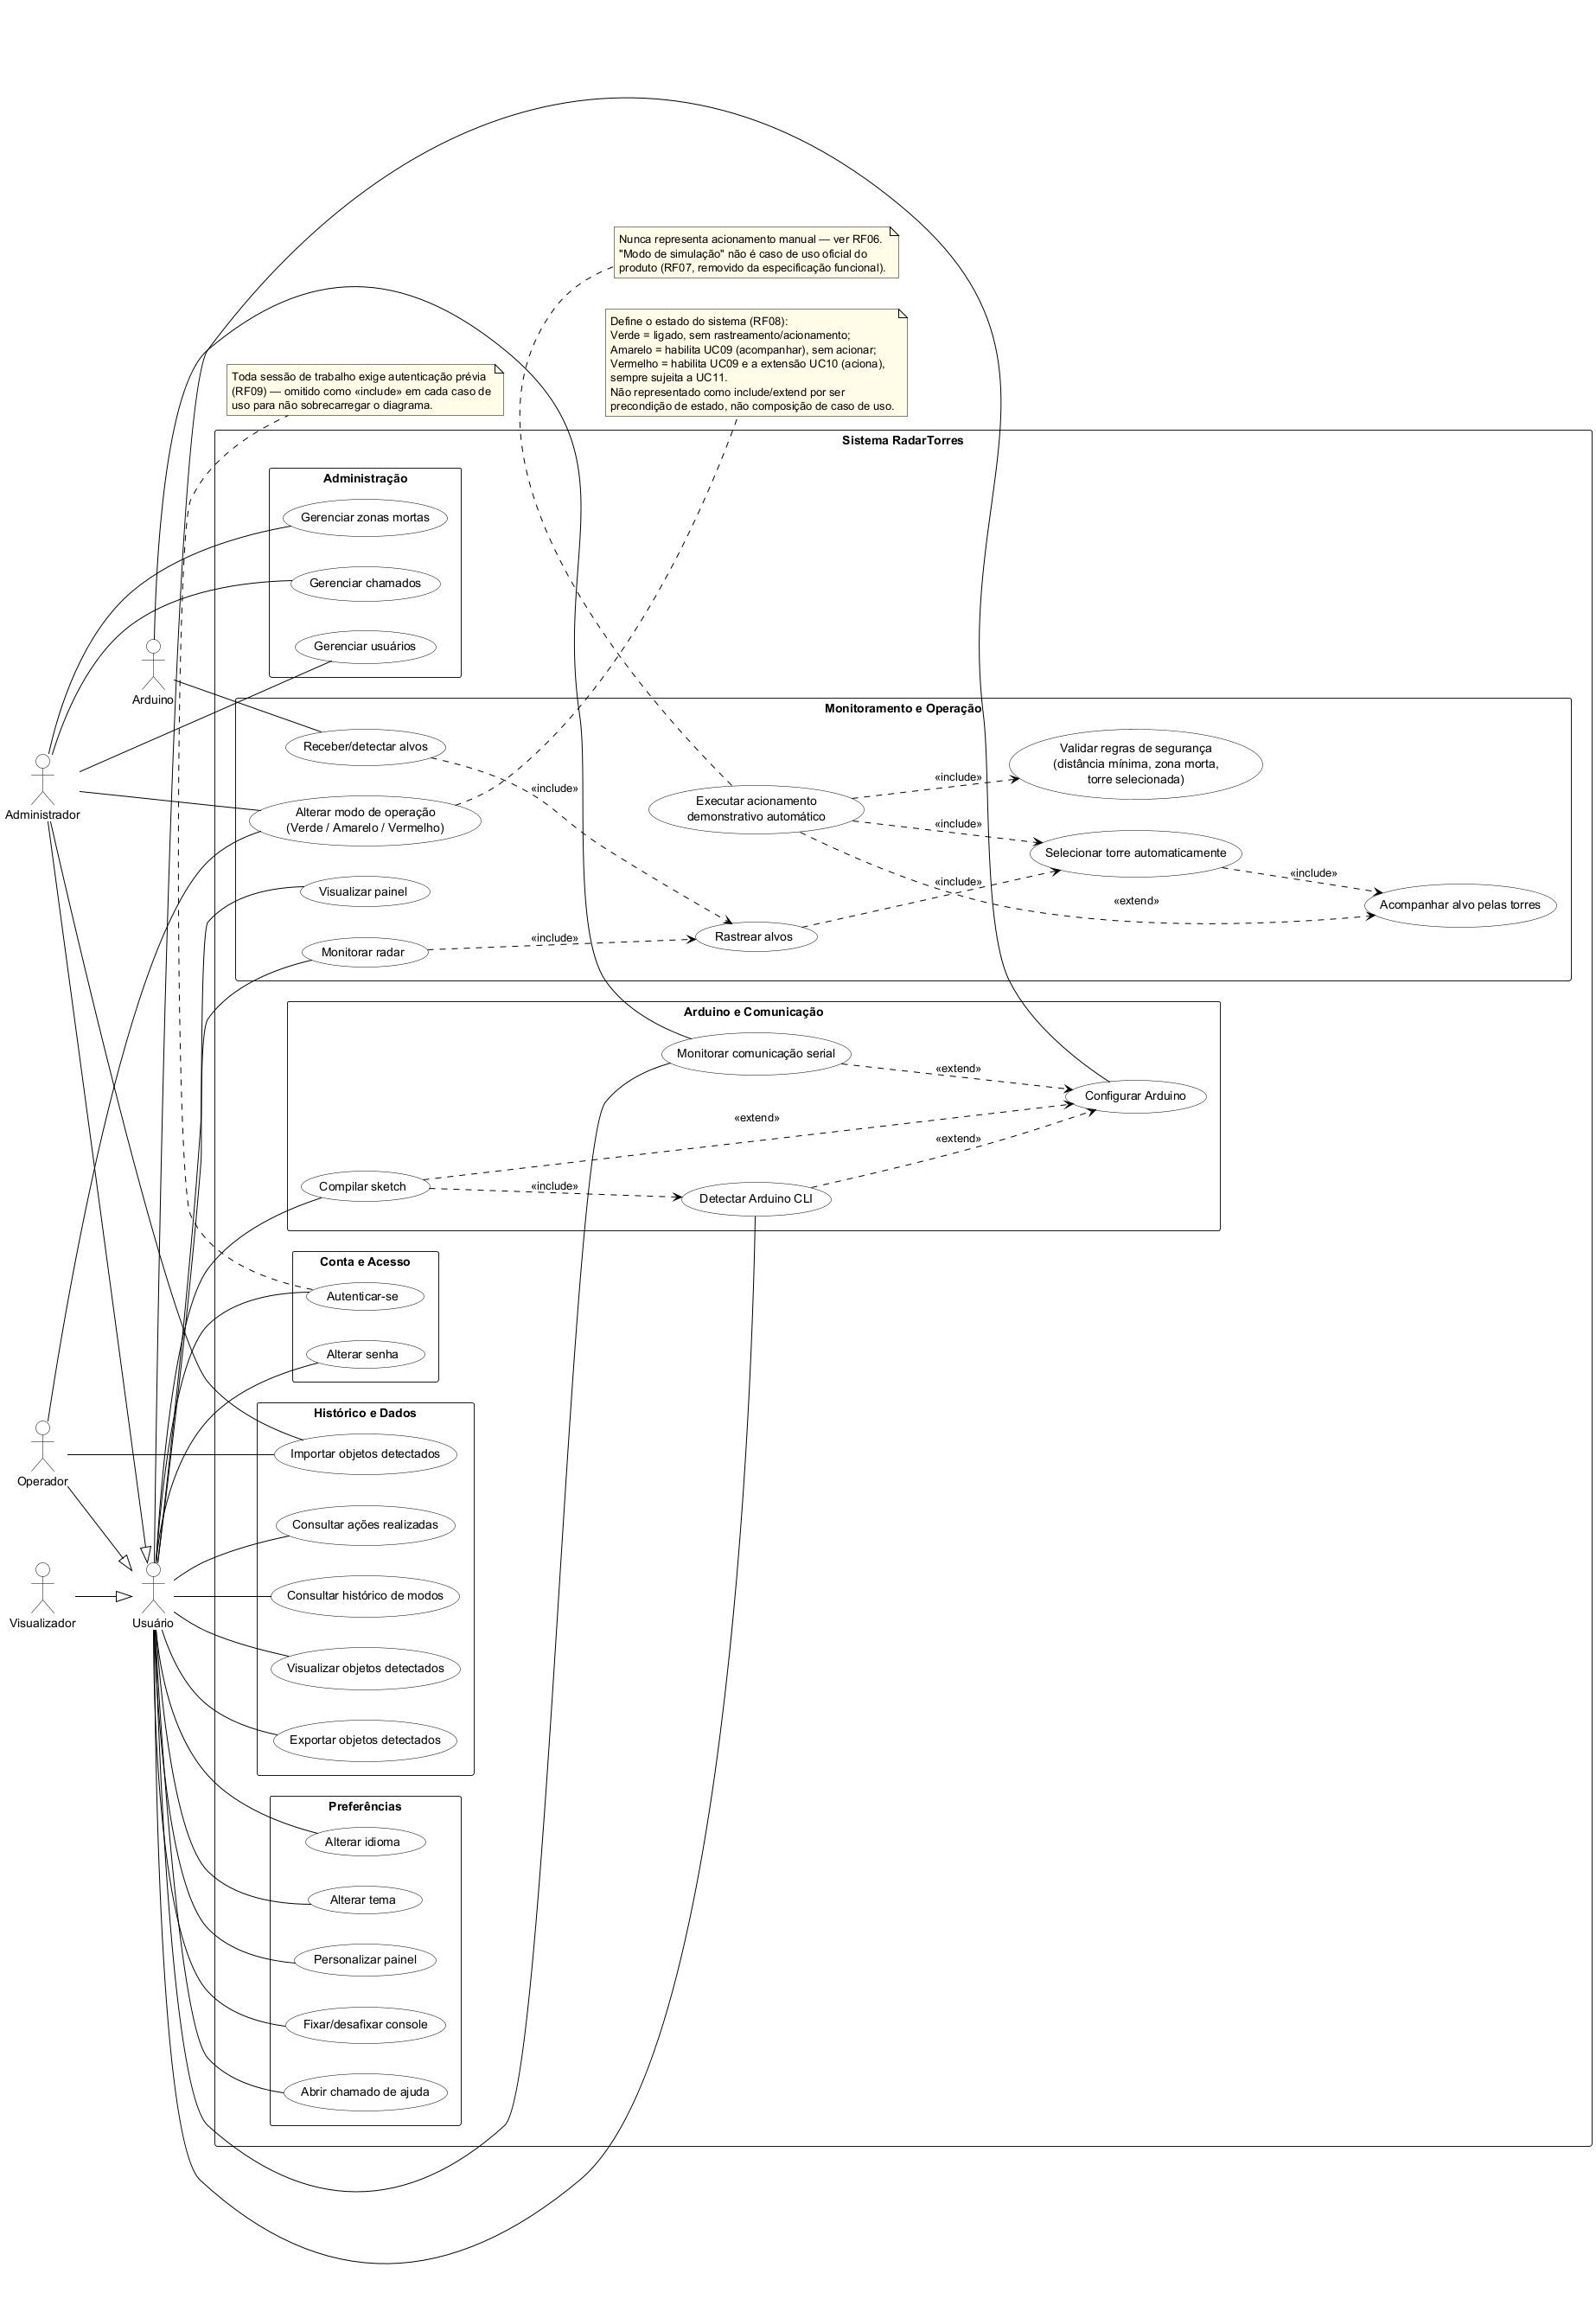
\includegraphics[width=\textwidth]{Diagrama_Casos_de_Uso.png}
  \caption{Diagrama de casos de uso do RadarTorres.}
  \label{fig:uc}
\end{figure}

\section{Especificação Resumida dos Casos de Uso}

\begin{longtable}{p{1.0cm}p{6.6cm}p{3.3cm}p{2.3cm}}
  \caption{Casos de uso do RadarTorres} \label{tab:uc} \\
  \hline
  \textbf{ID} & \textbf{Caso de Uso} & \textbf{Atores} & \textbf{Requis.} \\
  \hline
  \endfirsthead
  \multicolumn{4}{c}{\small \tablename~\thetable\ (continuação)} \\
  \hline
  \textbf{ID} & \textbf{Caso de Uso} & \textbf{Atores} & \textbf{Requis.} \\
  \hline
  \endhead
  \hline
  \endfoot
  \small
  UC01 & Autenticar-se & Usuário & RF08 \\
  UC02 & Alterar senha & Usuário & RF10 \\
  UC03 & Visualizar painel & Usuário & RF21 \\
  UC04 & Monitorar radar & Usuário & RF04 \\
  UC05 & Receber/detectar alvos & Arduino, Sistema & RF01, RF02 \\
  UC06 & Rastrear alvos & --- (automático) & RF03 \\
  UC07 & Selecionar torre automaticamente & --- (automático) & RF05 \\
  UC08 & Alterar modo de operação (Verde/Amarelo/Vermelho) & Administrador, Operador & RF07 \\
  UC09 & Acompanhar alvo pelas torres & --- (automático) & RF06, RF07 \\
  UC10 & Executar acionamento demonstrativo automático & --- (automático) & RF06 \\
  UC11 & Validar regras de segurança & --- (automático) & RF06, RNF04, RNF05, RF23 \\
  UC12 & Visualizar objetos detectados & Usuário & RF11, RF12 \\
  UC13 & Exportar objetos detectados & Usuário & RF13 \\
  UC14 & Importar objetos detectados & Administrador, Operador & RF14 \\
  UC15 & Consultar ações realizadas & Usuário & RF15 \\
  UC16 & Consultar histórico de modos & Usuário & RF16 \\
  UC17 & Gerenciar usuários & Administrador & RF17 \\
  UC18 & Gerenciar zonas mortas & Administrador & RF23 \\
  UC19 & Alterar idioma & Usuário & RF18 \\
  UC20 & Alterar tema & Usuário & RF18 \\
  UC21 & Personalizar painel & Usuário & RF21 \\
  UC22 & Fixar/desafixar console & Usuário & RF22 \\
  UC23 & Abrir chamado de ajuda & Usuário & RF19 \\
  UC24 & Gerenciar chamados & Administrador & RF20 \\
  UC25 & Configurar Arduino & Usuário & RF25 \\
  UC26 & Detectar Arduino CLI & Usuário & RF24 \\
  UC27 & Compilar sketch & Usuário & RF24 \\
  UC28 & Monitorar comunicação serial & Usuário, Arduino & RF25 \\
\end{longtable}

\textbf{RF09} (Controle de acesso por perfil) é o único requisito funcional válido sem caso de uso
próprio: não é uma ação que um ator realiza, é a regra que decide quais casos de uso cada ator
vê/executa, representada estruturalmente nas associações diferenciadas por perfil do diagrama.

\section{Relacionamentos entre Casos de Uso}

Os principais relacionamentos \emph{include}/\emph{extend} do diagrama são: UC04 e UC05 incluem
UC06 (Rastrear alvos); UC06 inclui UC07 (Selecionar torre); UC07 inclui UC09 (Acompanhar alvo);
UC10 estende UC09 e inclui UC07 e UC11 (Validar regras de segurança); UC27 inclui UC26 (Detectar
CLI); e UC26, UC27 e UC28 estendem UC25 (Configurar Arduino). Esses relacionamentos evitam
duplicar, em cada caso de uso, comportamento comum a vários fluxos.

\section{Conclusão}

Os 28 casos de uso especificados cobrem a totalidade dos requisitos funcionais do RadarTorres,
organizados em 6 agrupamentos (Conta e Acesso, Monitoramento e Operação, Histórico e Dados,
Administração, Preferências, Arduino e Comunicação). Os relacionamentos de \emph{include} e
\emph{extend} evidenciam o fluxo central automático do sistema — da recepção de uma leitura do
Arduino até o acionamento demonstrativo, sempre sujeito à validação de segurança —, enquanto os
casos de uso com ator humano cobrem autenticação, consulta/gestão de dados, preferências e
configuração do ambiente Arduino.
